% Introduction
This section describes the technologies used to query, cache, and process data in this project. The query engine refers mainly to Apache Spark and DuckDB, but the other technologies presented in this chapter operate at the same abstraction level while having different functions.

\subsection{Apache Spark}

Apache Spark (from now on simply Spark) is an open-source distributed computing framework designed to handle large-scale data-intensive applications~\cite{zahariaApacheSparkUnified2016}. Spark builds from the roots of MapReduce and its variants. MapReduce is a distributed programming model first designed by Google that enables the management of large datasets~\cite{dean2004mapreduce}. The paradigm was later implemented as an open-source project by Yahoo! engineers under the name of Hadoop MapReduce~\cite{borthakurHadoopDistributedFile2005}. Spark improved this approach using \glspl{RDD}~\cite{Zaharia:EECS-2011-82}. \glspl{RDD} are a distributed memory abstraction that enables a lazy in-memory computation tracked through lineage graphs, ultimately increasing fault tolerance~\cite{Zaharia:EECS-2011-82}. The difference between Hadoop MapReduce and Spark is represented in Figure~\ref{fig:MapReducevsSpark}.

\begin{figure}[!ht]
  \begin{center}
    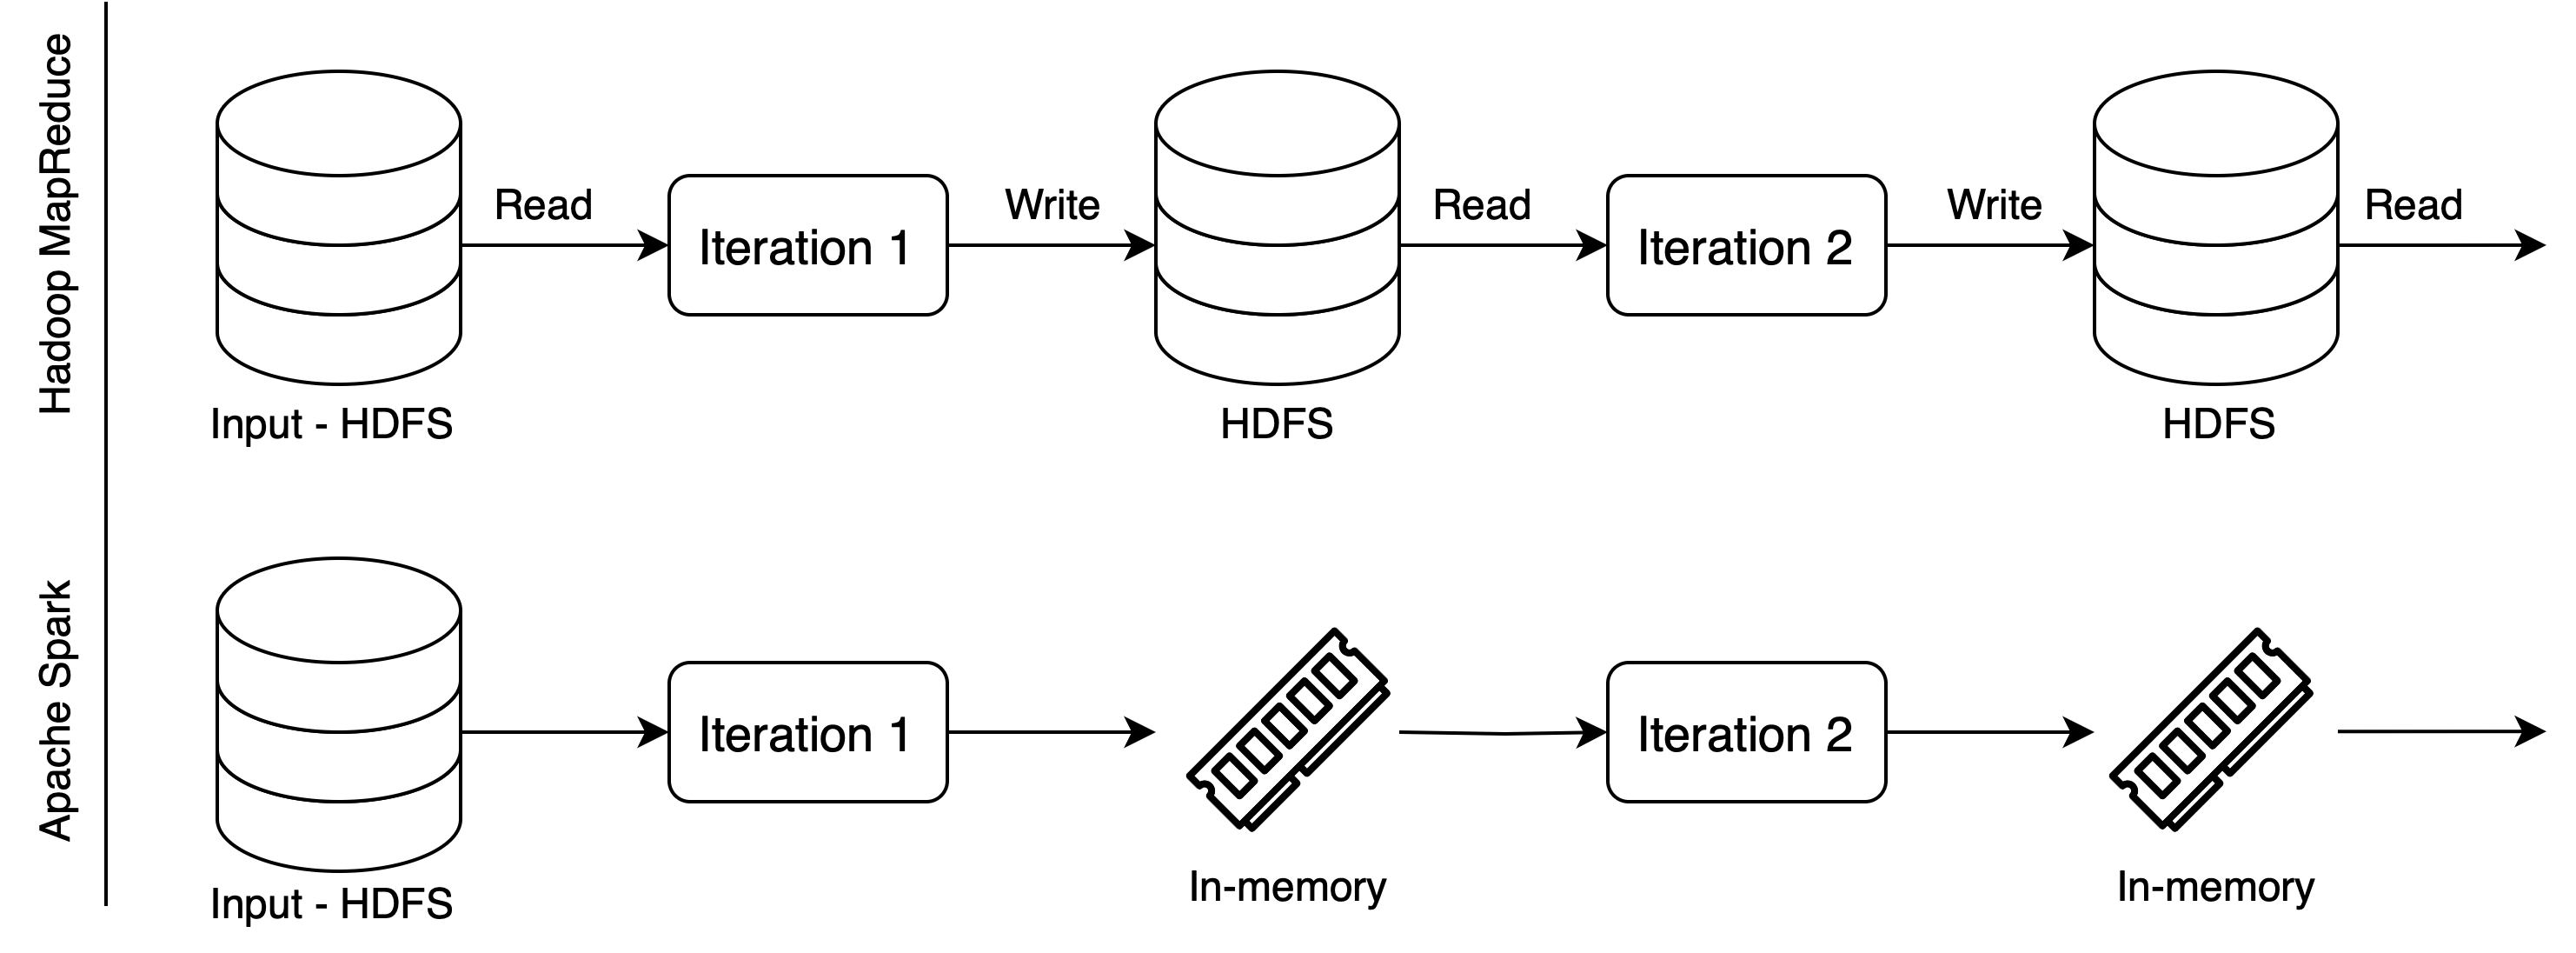
\includegraphics[width=\textwidth]{figures/2-background/Spark_MapReduce.png}
  \end{center}
  \caption[Hadoop MapReduce vs. Apache Spark]{Hadoop MapReduce and Apache Spark execution differences. Apache Spark enables fast in-memory computation instead of continuously saving and loading data from disks as Hadoop MapReduce. Diagram inspired by the Data-intensive Computing lectures at KTH by Prof. A. H. Payberah. Course website available at \url{https://www.kth.se/student/kurser/kurs/ID2221?l=en}.}
  \label{fig:MapReducevsSpark}
\end{figure}

\subsection{Apache Kafka}

Apache Kafka (from now on, Kafka) is an open-source distributed data streaming platform designed for high-throughput and scalable data processing~\cite{krepsKafkaDistributedMessaging2011}. Kafka is most typically used for real-time streaming applications thanks to low latency. 

\begin{figure}[!ht]
    \begin{center}
      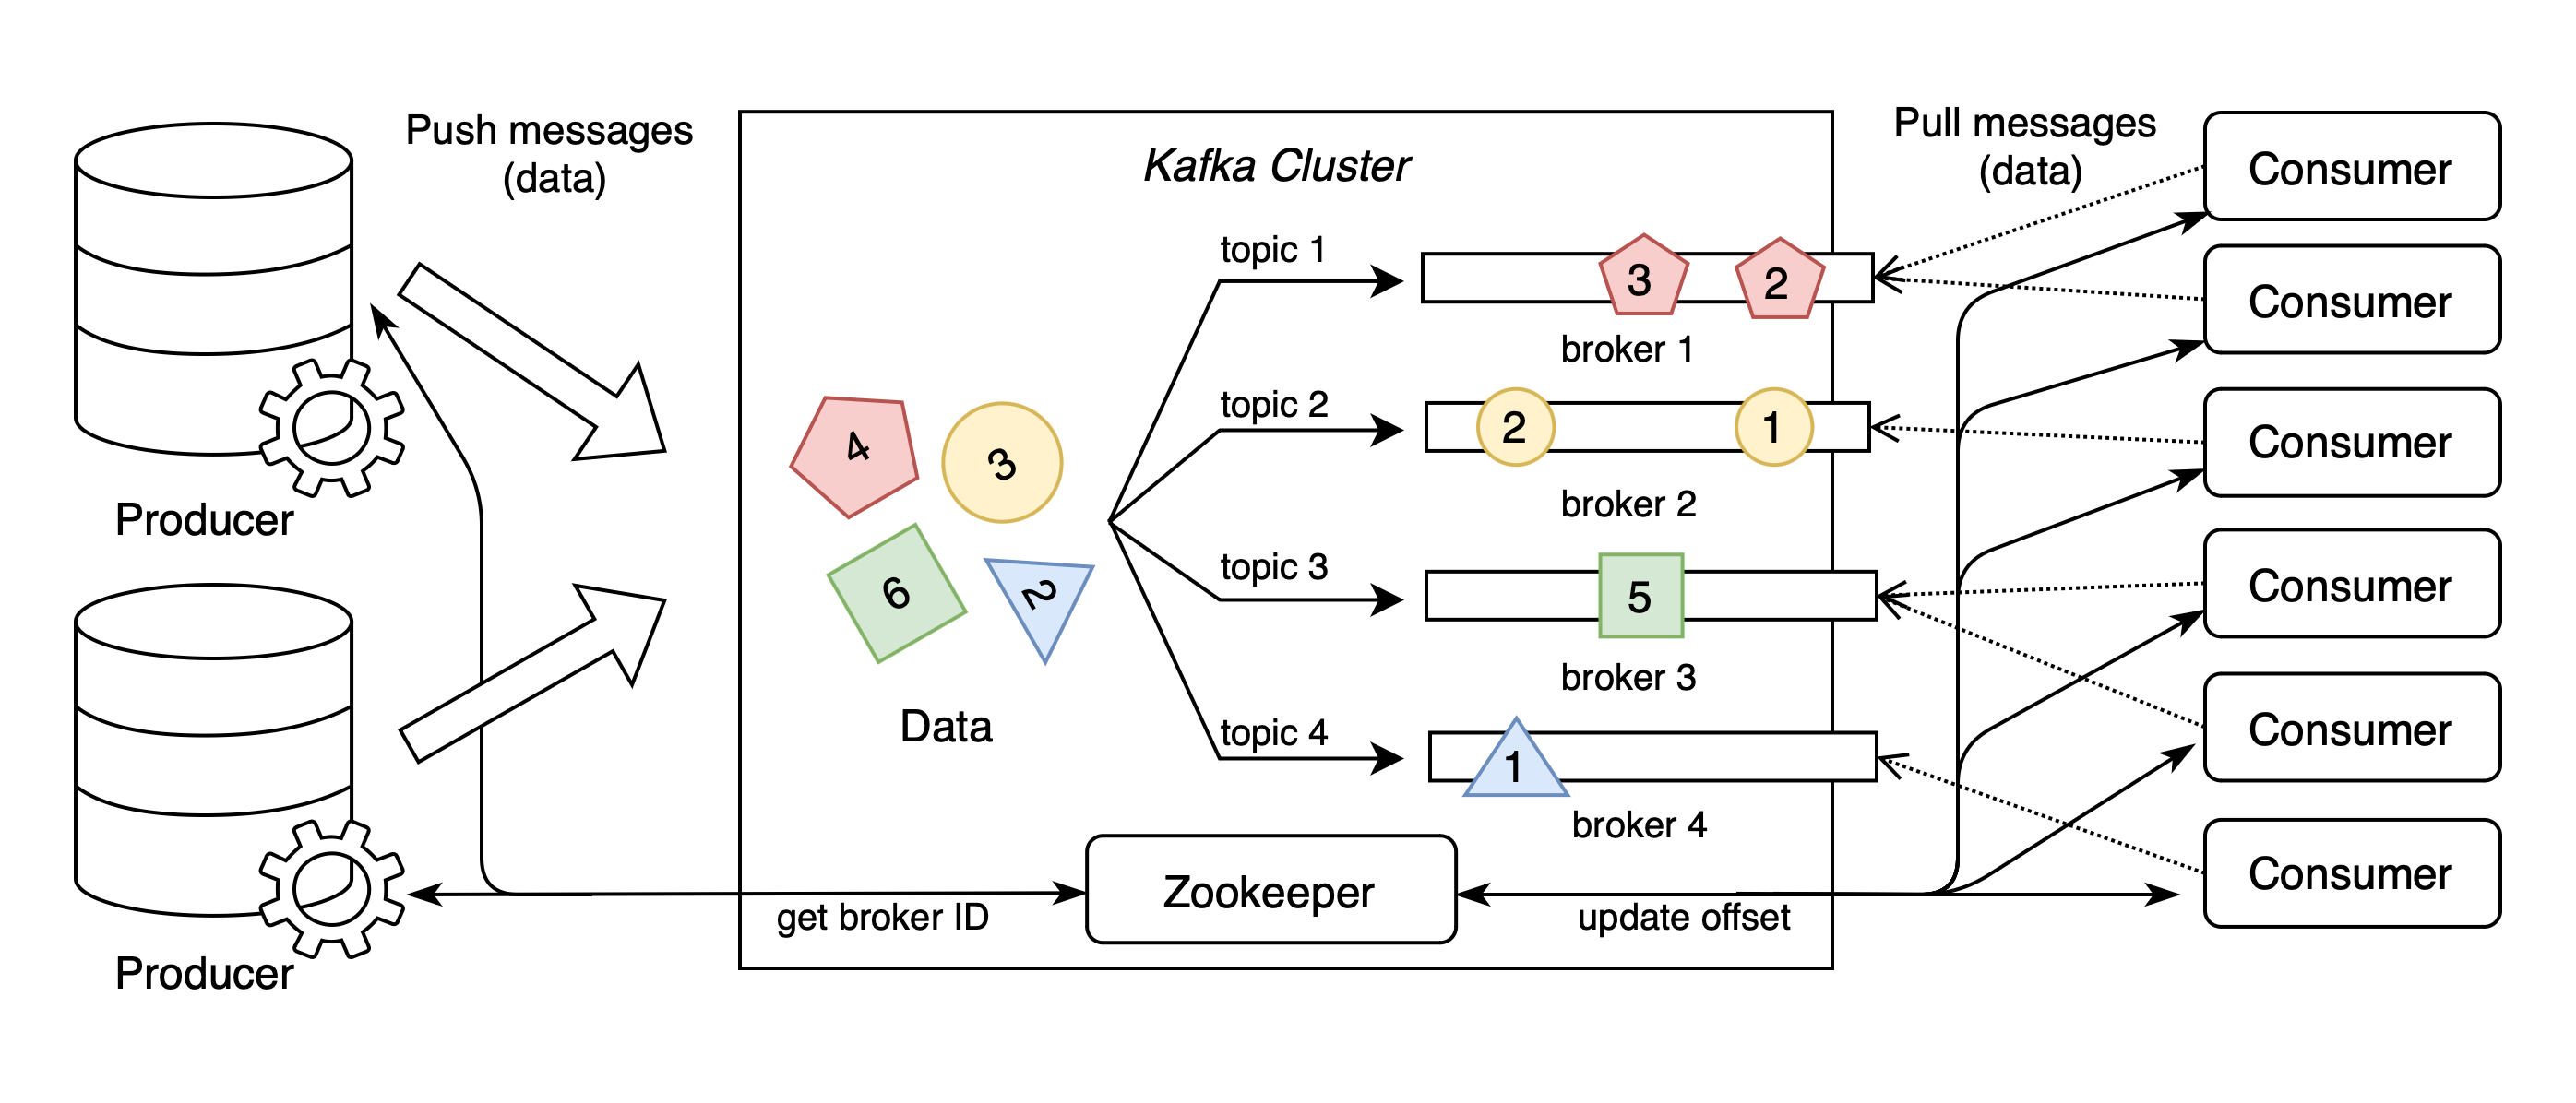
\includegraphics[width=\textwidth]{figures/2-background/kafka.png}
    \end{center}
    \caption[Kafka architecture]{Kafka architecture. A shape and a color characterize messages associated with a topic. Note: in Kafka, messages on different topics are replicated across different brokers and are not represented in the image for simplicity. It is to be noted that for each topic, a broker is elected as the leader while the other brokers replicate its contents. Diagram inspired by DoubleCloud article available at \url{https://double.cloud/blog/posts/2023/03/the-many-use-cases-of-apache-kafka/}.}
    \label{fig:kafka}
\end{figure}

Figure \ref{fig:kafka} shows the components and messages exchanged in a Kafka cluster. The key components of Kafka are:
\begin{enumerate}
    \item \textbf{Producer}: an application that produces and labels data with specific topics (shapes in the figure).
    \item \textbf{Zookeeper}: responsible for keeping track of brokers and the topic's current offset.
    \item \textbf{Broker}: a computational node (or server) that handles data on a specific topic. It is responsible for receiving messages from producers. Once messages are received, the broker forwards them upon request by the consumers. This mechanism enables the asynchronous protocol.
    \item \textbf{Consumer}: an application interested in topic-specific data. To access data, it is subscribed to a topic and receives new messages when published. More consumers can subscribe to a topic.
\end{enumerate}

The protocol allows applications acting as producers and consumers to avoid having a synchronous protocol. This feature enables producers to achieve high throughput since they can send messages without waiting for consumers to process them. Additionally, this allows consumers to be flexible with workload size.

Given its distributed nature, Kafka allows several producers, consumers, and brokers to exist simultaneously. This feature enables the system to be tuned according to the needs of a specific application. 

\subsection{DuckDB}

DuckDB \cite{raasveldtDuckDBEmbeddableAnalytical2019} is an open-source, embedded, \gls{OLAP} \gls{DBMS}. DuckDB was designed to process small quantities of data (1 - 100 GBs) within the same process or application that runs it instead of a different process/application. These features create an efficient \gls{OLAP} database that can be used for data analysis and data processing on a small scale, without the complexity of a more complex \gls{DBMS}, e.g., Teradata \cite{shahImproveYourOLAP}. 

The light structure that characterizes DuckDB enables this system to be highly responsive with low latency. The system's limitations regard data size. As DuckDB uses in-memory processing, it cannot handle big workloads (1TB or more) requiring disk loads.

\subsection{Arrow Flight}

Arrow Flight is a high-performance framework for data transfer over a network, typically Arrow tables \cite{wesmIntroducingApacheArrow2019}. This protocol enables the transfer of large quantities of data stored in a format, e.g., Arrow tables, without having to serialize or deserialize it for transfer. This greatly speeds up the data transfer, making Arrow Flight extremely efficient. Arrow Flight is designed to be cross-platform and has support for multiple programming languages (C++, Python, Java). The protocol also supports parallelism, speeding up transfers using multiple nodes on parallel systems. Arrow Flight protocol is built on top of gRPC, enabling standardization and easier development of connectors. 